\documentclass[11pt,a4paper]{article}

\usepackage[utf8]{inputenc}
\usepackage[T1]{fontenc}
\usepackage[english]{babel}
\usepackage{geometry}
\usepackage{graphicx}
\usepackage{booktabs}
\usepackage{float}
\usepackage{hyperref}
\usepackage{amsmath}

\geometry{margin=2.5cm}

\begin{document}

\begin{titlepage}
    \centering

    \vspace*{2cm}

    {\Large Universidad de Las Palmas de Gran Canaria\par}

    \vspace{0.5cm}

    {\large Degree in Data Science and Engineering\par}

    \vspace{0.5cm}

    {\large Big Data\par}

    \vfill

    {\Huge\bfseries Assignment 1\par}

    \vspace{0.5cm}

    {\LARGE Basic Matrix Multiplication in Python, Java and C\par}

    \vfill

    {\large Student: María Báez Marrero\par}

    \vspace{0.5cm}

    {\large Academic Year 2026--2027\par}

    \vspace{1cm}

\end{titlepage}

\begin{abstract}

This assignment compares basic dense matrix multiplication implementations in Python, Java and C using the same standard triple-loop algorithm and identical input matrices.

Execution time is measured for matrix sizes from 50 to 250 using five repetitions per configuration, summarized with the median and interquartile range. Peak Resident Set Size (Peak RSS) is used as the memory metric.

Correctness is verified using known test cases, identity and zero matrices, cross-language checksums, and NumPy as a trusted reference implementation.

At $n=250$, the median execution time was approximately 1.06 s for Python, 12.7 ms for Java and 19.5 ms for C. Peak RSS at the same size was approximately 21.4 MB for Python, 55.9 MB for Java and 2.1 MB for C.

The results show that the three implementations have the same theoretical $O(n^3)$ algorithmic structure but substantially different observed runtime and memory behaviour under the tested execution environment.

The estimated log-log slopes were approximately 3.02 for Python, 3.15 for C and 2.10 for Java, showing behaviour close to the expected cubic model for Python and C over the tested range.

\end{abstract}
\section{Introduction}

Matrix multiplication is a fundamental operation in scientific computing, data processing and machine learning. Although the underlying algorithm may be identical, its practical performance can differ considerably depending on the programming language, runtime environment, memory representation and compiler or interpreter.

The objective of this assignment is to compare straightforward dense matrix multiplication implementations written in Python, Java and C under controlled experimental conditions.

The research question is:

\begin{quote}
How do execution time and memory usage differ when the same basic dense matrix multiplication algorithm is implemented in Python, Java and C on the same hardware and using the same input matrices?
\end{quote}

The hypothesis is that execution time will increase approximately according to the cubic growth of the standard matrix multiplication algorithm as matrix size increases. Differences are also expected between the three implementations because Python, Java and C use different execution and memory models.

\section{Background}

The standard dense matrix multiplication algorithm computes each element of the result matrix as

\[
C_{ij} = \sum_{k=1}^{n} A_{ik}B_{kj}.
\]

For two square matrices of size $n \times n$, the straightforward triple-loop algorithm performs arithmetic work proportional to $n^3$, giving a theoretical time complexity of $O(n^3)$ \cite{cormen2022}.

Practical performance, however, depends not only on asymptotic complexity but also on the execution environment, memory representation, compiler optimizations and runtime behaviour.

Java benchmarking requires particular care because Just-in-Time compilation, garbage collection and other JVM effects can influence measurements \cite{georges2007}. More generally, seemingly minor experimental choices can introduce performance-measurement bias \cite{mytkowicz2009}.

For Python measurements, \texttt{time.perf\_counter()} is used because it provides a high-resolution performance counter suitable for measuring short durations \cite{python_time}.

\section{Methodology}

\subsection{Implementations}

The matrix multiplication algorithm is implemented in Python, Java and C using the same loop order:

\[
i \rightarrow j \rightarrow k.
\]

No optimized matrix multiplication libraries such as NumPy or BLAS are used in the benchmarked implementations.

Python stores matrices as lists of lists of Python integers. Java uses two-dimensional \texttt{int[][]} arrays. C uses dynamically allocated matrices with integer pointers.

The implementations are sequential and do not explicitly use multithreading.

\subsection{Input Data}

The tested matrix sizes are:

\[
50,\ 100,\ 150,\ 200,\ 250.
\]

All matrix values are integers between 0 and 9.

The matrices are generated once using Python with random seed 42 and stored as CSV files. The same input files are read by Python, Java and C so that all implementations process identical data.

With the selected value range and maximum size, the maximum possible value of one output element is

\[
250 \times 9 \times 9 = 20250,
\]

which remains well within the integer range used by Java and C.

\subsection{Correctness Validation}

Correctness is checked using three types of tests:

\begin{itemize}
    \item matrices with a known multiplication result,
    \item multiplication by the identity matrix,
    \item multiplication by the zero matrix.
\end{itemize}

The implementations also calculate a checksum of the resulting matrix after each timed execution. For every matrix size, the checksum is identical in Python, Java and C.

In addition, the Python implementation is compared against NumPy's matrix multiplication as a trusted reference implementation. All tested matrix sizes produced matching results.

\subsection{Runtime Measurement}

Each matrix size is executed five times for each language.

Input loading and allocation of the output matrix are excluded from the timed region.

Inside the timed region, each output element is initialized and the standard multiplication kernel is executed.

The checksum is calculated after the timer stops, so checksum computation does not affect the measured runtime.

The timers used are:

\begin{itemize}
    \item Python: \texttt{time.perf\_counter()},
    \item Java: \texttt{System.nanoTime()},
    \item C: \texttt{CLOCK\_MONOTONIC}.
\end{itemize}

Java performs three untimed warm-up executions for each matrix size before the measured repetitions.

The C implementation is compiled using Apple Clang with optimization level \texttt{-O2}.

For every language and matrix size, the median execution time and interquartile range (IQR) are reported.

\subsection{Memory Measurement}

Memory usage is measured using Peak Resident Set Size (Peak RSS).

On macOS, Peak RSS is collected using:

\begin{verbatim}
/usr/bin/time -l
\end{verbatim}

The metric represents the peak memory usage of the complete process. Therefore, it includes runtime overhead such as the Python interpreter and the Java Virtual Machine.

One Peak RSS measurement is recorded for every language and matrix size.

\subsection{Experimental Environment}

The experiments were executed on a MacBook Pro with:

\begin{itemize}
    \item Apple M4 processor,
    \item 10 CPU cores,
    \item 16 GB RAM,
    \item macOS 26.3.1,
    \item ARM64 architecture.
\end{itemize}

Software versions include:

\begin{itemize}
    \item Python 3.13.0,
    \item OpenJDK 25.0.2,
    \item Apple Clang 21.0.0,
    \item pandas 3.0.0,
    \item matplotlib 3.10.8.
\end{itemize}

The final experimental scope is limited to matrix sizes up to $n=250$. A practical runtime budget of 5 seconds per individual multiplication and a Peak RSS budget of 1 GB are used as feasibility limits.

Although the predefined runtime budget was 5 seconds per multiplication, the experiment was intentionally limited to $n=250$ in order to keep the comparison common across all three languages and to maintain a compact and inspectable dataset. Therefore, $n=250$ is the largest tested size in this study, not the computational limit of the machine.

\section{Results}

\subsection{Correctness Results}

All three implementations produced identical checksums for every tested matrix size. In addition, the complete result matrices produced by the Python implementation matched NumPy exactly. Java and C were validated through the same input matrices, correctness tests and matching cross-language checksums.

\begin{table}[H]
\centering
\caption{Cross-language checksum validation and NumPy reference comparison.}
\label{tab:correctness}
\begin{tabular}{rrc}
\toprule
$n$ & Checksum & NumPy match \\
\midrule
50  & 2580329   & Yes \\
100 & 20043070  & Yes \\
150 & 68563585  & Yes \\
200 & 161354779 & Yes \\
250 & 315567802 & Yes \\
\bottomrule
\end{tabular}
\end{table}

Because the experiment uses integer arithmetic and all values remain within the representable range, correctness comparison is exact and no numerical tolerance is required.
\subsection{Execution Time}

Table~\ref{tab:runtime} summarizes the median execution time and IQR for every language and matrix size.

\begin{table}[H]
\centering
\caption{Median execution time and interquartile range in seconds.}
\label{tab:runtime}
\begin{tabular}{rrrrrrr}
\toprule
$n$ & Py Med. & Py IQR & Java Med. & Java IQR & C Med. & C IQR \\
\midrule
50  & 0.008169 & 0.000141 & 0.000432 & 0.000009 & 0.000069 & $2.0\times10^{-9}$ \\
100 & 0.067900 & 0.015727 & 0.001090 & 0.000194 & 0.000691 & 0.000077 \\
150 & 0.231970 & 0.004558 & 0.003211 & 0.000288 & 0.002257 & 0.000227 \\
200 & 0.543361 & 0.008861 & 0.006495 & 0.000168 & 0.009325 & 0.000052 \\
250 & 1.055285 & 0.028924 & 0.012666 & 0.000114 & 0.019843 & 0.000311 \\
\bottomrule
\end{tabular}
\end{table}

\subsection{Comparison with the Cubic Model}

To compare the measurements with the expected $O(n^3)$ model, the median execution time was normalized by $n^3$.

\begin{table}[H]
\centering
\caption{Median execution time normalized by $n^3$.}
\label{tab:normalized}
\begin{tabular}{rrrr}
\toprule
$n$ & Python & Java & C \\
\midrule
50  & $6.53\times10^{-8}$ & $3.46\times10^{-9}$ & $5.52\times10^{-10}$ \\
100 & $6.79\times10^{-8}$ & $1.09\times10^{-9}$ & $6.91\times10^{-10}$ \\
150 & $6.87\times10^{-8}$ & $9.51\times10^{-10}$ & $6.69\times10^{-10}$ \\
200 & $6.79\times10^{-8}$ & $8.12\times10^{-10}$ & $1.17\times10^{-9}$ \\
250 & $6.75\times10^{-8}$ & $8.11\times10^{-10}$ & $1.27\times10^{-9}$ \\
\bottomrule
\end{tabular}
\end{table}

For Python, the normalized execution time remains almost constant across the tested sizes. This is consistent with the expected cubic growth of the standard triple-loop algorithm.

C also remains within approximately the same order of magnitude, although the normalized cost increases for the largest tested sizes.

Java shows a different pattern. Its normalized execution time decreases substantially between the smallest and largest tested matrices, indicating that runtime effects influence the measurements for small matrix sizes.

The log-log slope is estimated using

\[
p = \frac{\ln(T_{250}/T_{50})}{\ln(250/50)},
\]

where $T_n$ is the median execution time for matrix size $n$.

A simple log-log slope estimate between the smallest and largest tested sizes gives approximately 3.02 for Python, 3.52 for C and 2.10 for Java.
Python and C are therefore close to the theoretical cubic exponent of 3 over the tested range. The lower Java slope indicates that the observed Java timings are affected by additional runtime effects, particularly for the smaller matrix sizes.

\begin{figure}[H]
\centering
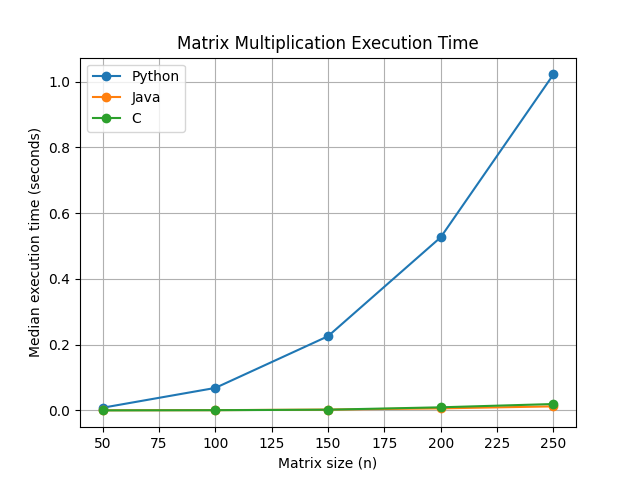
\includegraphics[width=0.8\textwidth]{figures/execution_time.png}
\caption{Median execution time over five measured repetitions for Python, Java and C. Error bars represent the interquartile range.}
\label{fig:execution}
\end{figure}

Because Python execution times are much larger than those of Java and C, a logarithmic scale helps distinguish the lower execution times more clearly.

\begin{figure}[H]
\centering
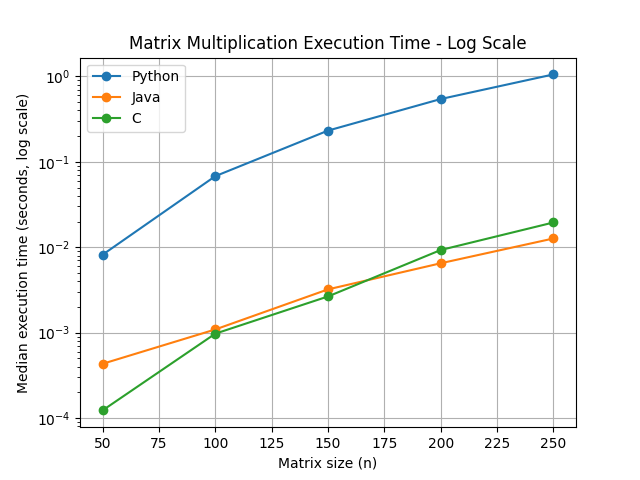
\includegraphics[width=0.8\textwidth]{figures/execution_time_log.png}
\caption{Median execution time over five measured repetitions using a logarithmic vertical scale. Error bars represent the interquartile range.}
\label{fig:execution_log}
\end{figure}

\subsection{Memory Usage}

Table~\ref{tab:memory} summarizes the measured Peak RSS values.

\begin{table}[H]
\centering
\caption{Peak RSS memory usage in MB ($10^6$ bytes).}
\label{tab:memory}
\begin{tabular}{rrrr}
\toprule
$n$ & Python & Java & C \\
\midrule
50  & 17.42 & 43.02 & 1.33 \\
100 & 17.99 & 44.73 & 1.46 \\
150 & 18.83 & 46.84 & 1.61 \\
200 & 20.04 & 51.30 & 1.85 \\
250 & 21.41 & 55.93 & 2.08 \\
\bottomrule
\end{tabular}
\end{table}

\begin{figure}[H]
\centering
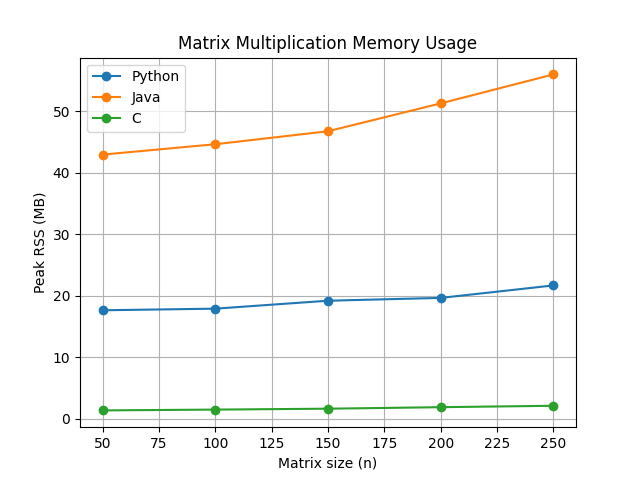
\includegraphics[width=0.8\textwidth]{figures/memory_usage.png}
\caption{Peak RSS memory usage for the three implementations.}
\label{fig:memory}
\end{figure}

\section{Discussion}

The results show substantial runtime differences between the three implementations.

Python is consistently slower than Java and C for every tested matrix size. In Python, matrices are stored as lists of references to Python integer objects rather than as contiguous primitive integer arrays. This introduces additional interpreter and object-management overhead and can reduce memory locality.

Java and C show much smaller execution times and are closer to each other. C has the lowest median execution time for the smallest tested sizes, while Java produces lower median times for the larger tested sizes of 200 and 250. These observations are specific to the tested hardware, compiler settings, JVM version and implementation and should not be interpreted as universal language rankings.

The fact that Java becomes faster than C for the largest tested sizes is an observed result, but its exact cause was not isolated in this experiment. Possible explanations include differences in JIT optimization, array handling and memory-access behaviour. Further experiments would be required to determine the cause.

The normalized runtime analysis provides additional evidence about the growth trend. Python shows an almost constant normalized execution time and an estimated log-log slope of approximately 3.02, which is very close to the theoretical cubic exponent. C produces a higher estimated slope of approximately 3.52. This still reflects strong superlinear growth, but the deviation from 3 indicates that constant factors and memory-access effects influence the measurements over the limited tested range.

The increase in normalized cost observed for C at the largest sizes may also be influenced by cache and memory-access effects, particularly because matrix $B$ is accessed by columns in the chosen $i \rightarrow j \rightarrow k$ loop order. This was not measured directly and is therefore only a possible explanation.

Java behaves differently over the tested range, with an estimated slope of approximately 2.10. The smallest Java measurements have a relatively high normalized cost, while the values stabilize for larger matrices. This suggests that JVM runtime effects and JIT compilation influence the measurements at small sizes. Therefore, the Java measurements should not be interpreted as a clean empirical estimate of the asymptotic exponent over this limited range.

The Peak RSS measurements show a different pattern from the execution-time results.

Between $n=50$ and $n=250$, measured Peak RSS increased from approximately 17.4 MB to 21.4 MB for Python, from 43.0 MB to 55.9 MB for Java, and from 1.33 MB to 2.08 MB for C.

This corresponds to an increase of approximately 4.0 MB for Python, 12.9 MB for Java and 0.75 MB for C.

The C increase is close to the theoretical storage increase expected for three dense matrices containing 32-bit integers. At $n=250$, three matrices require approximately

\[
3 \times 250^2 \times 4 = 750000
\]

bytes of element storage.

Python and Java show substantially larger process-level memory usage because Peak RSS measures the complete process rather than only the matrix data. The Python measurement includes interpreter and object-management overhead. The Java result includes JVM, heap and runtime overhead, and may also include temporary objects created while parsing the CSV input files.

Therefore, these Peak RSS values should not be interpreted as direct measurements of matrix storage alone.

The experiment also has several limitations. Only one computer and one software environment are tested. Memory is measured once for each configuration rather than repeatedly. The matrix sizes are limited to 250, and different runtime environments introduce unavoidable asymmetries such as JIT compilation in Java and ahead-of-time optimization in C.

\section{Conclusions}

This experiment compared basic dense matrix multiplication implementations in Python, Java and C using shared inputs and the same triple-loop algorithm.

All implementations produced correct and equivalent results, confirmed through basic correctness tests, cross-language checksums and comparison with NumPy.

The measured execution times show that Python is substantially slower than Java and C for the tested configurations. Java and C exhibit much lower execution times, with their relative performance varying across matrix sizes.

Peak RSS measurements show that Java uses the largest amount of process-level memory, while C uses the least in the tested environment. These differences reflect not only matrix storage but also runtime and process overhead.

Overall, the results demonstrate that identical algorithmic complexity does not imply identical practical performance. Language runtime, memory representation, compiler optimization and execution environment all influence observed behaviour.

The study does not determine why Java becomes faster than C for the largest tested sizes, nor does it establish behaviour for substantially larger matrices. These questions remain open for future experiments.

\section{Reproducibility Materials}

The complete project is available at:

\url{https://github.com/mariabaezz/big-data-assignment1}

The repository contains the source code, shared input matrices, raw CSV measurements, analysis scripts, figures, environment information and README. The README includes the exact commands required to reproduce the experiments and figures.

\section*{Use of Generative AI}

Claude was used as a support tool for explaining concepts, planning the experimental workflow, debugging, and revising the English wording of the documentation and report.

\bibliographystyle{plain}
\bibliography{references}

\end{document}